\documentclass[a4paper, 12pt]{article}
\usepackage[english]{babel}
\usepackage[utf8]{inputenc}
\usepackage[T1]{fontenc}
\usepackage{lmodern}

\usepackage{url}
\usepackage{graphicx}

\usepackage{amsmath}
\usepackage{amsthm}
\usepackage{amsfonts}
\usepackage{subfigure}

\textwidth 15cm
\textheight 24cm
\oddsidemargin.5cm
\evensidemargin.5cm
\topmargin-5mm
\addtolength{\footskip}{10pt}
\pagestyle{plain}

\addto\captionsenglish{\renewcommand{\refname}{Literatura}}

\usepackage{algorithm}
\usepackage{algpseudocode}
\renewcommand{\algorithmicrequire}{\textbf{Vhod:}}
\renewcommand{\algorithmicensure}{\textbf{Izhod:}}
\makeatletter
\renewcommand{\ALG@name}{Algoritem}
\makeatother

\addto\captionsenglish{\renewcommand{\figurename}{Slika}}


\theoremstyle{definition} % tekst napisan pokoncno
\newtheorem{definicija}{Definicija}[section]
\newtheorem{primer}[definicija]{Primer}
\addto\captionsenglish{\renewcommand\proofname{Dokaz}}
\newtheorem{opomba}[definicija]{Opomba}
\newtheorem{zgled}[definicija]{Zgled}

\theoremstyle{plain} % tekst napisan posevno
\newtheorem{lema}[definicija]{Lema}
%\newtheorem{zgled}[definicija]{Zgled}
\newtheorem{izrek}[definicija]{Izrek}
\newtheorem{trditev}[definicija]{Trditev}
\newtheorem{posledica}[definicija]{Posledica}

%\usepackage{graphicx}
\newtheorem{theorem}{Izrek}[section]
\newtheorem{definition}{Definicija}[section]
\newtheorem{corollary}{Posledica}[theorem]
\newtheorem{lemma}[theorem]{Lema}

\newcommand{\program}{Finančna matematika} 
\newcommand{\imeavtorja}{Lina Ivanova, Tia Krofel} 
\newcommand{\naslovdela}{Bernsteinovi bazni polinomi treh spremenljivk}
\newcommand{\letnica}{2023} 

\title{Bernstainovi baznih polinomov treh spremenljivk}
\author{Tia Krofel, Lina Ivanova}
\date{December 2023}

\begin{document}


\thispagestyle{empty}
\noindent{\large
UNIVERZA V LJUBLJANI\\[1mm]
FAKULTETA ZA MATEMATIKO IN FIZIKO
%\program\ -- 1.~stopnja
}
\vfill

\begin{center}{\large
\imeavtorja\\[2mm]
{\bf \naslovdela}\\[10mm]
Seminar pri predmetu Računalniško podprto (geometrijsko) oblikovanje\\[1cm]
%Mentorica: \imementorja
}
\end{center}
\vfill

\noindent{\large
Ljubljana, 2023}
\pagebreak

\section{Uvod}

V tem delu seminarja predstavimo Bernsteinove bazne polinome 
treh spremenljivk. Pri predmetu Računalniško podprto (geometrijsko)
oblikovanje smo spoznali Bernsteinove bazne polinome ene spremenljivke ter  
njihovo razširitev na dve spremenljivki.

Razlog za tako obširno obravnavo Bernsteinovih baznih polinomov leži v dejstvu, 
da lahko, v primerjavi z drugimi načini aproksimacije, z njihovo pomočjo 
pridemo do zelo dobrih približkov, pri čemer potrebujemo relativno majhno število 
kontrolnih točk. To je še posebej pomembno, če so naši računalniški viri omejeni 
ali pa želimo minimizirati število podatkov.

V nadaljevanju tako najprej predstavimo prostor polinomov,
kjer lahko operiramo s polinomi treh spremenljivk. Nato si ogledamo 
baricentrične koordinate za poljubno točko $(x,y,z)\in\mathbb{R}^3$ in kako izgleda 
kontrolna mreža, ki je v obliki strukture iz tetraedrov.
Zatem definiramo naslovni pojem, Bernsteinove bazne polinome 
treh spremenljivk. Za konec izpišemo še de Casteljaujev algoritem 
in si ogledamo smerne odvode vektorjev, ki so elementi prostora $\mathbb{R}^3$.

\section{Prostor $\mathbb{P}_n$}

Za začetek s $\mathbb{P}_n^3$ označimo prostor polinomov treh spremenljivk stopnje $n$, 
torej prostor končnih dimenzij z vsemi funkcijami oblike 

$$ p(x,y,z):=\sum_{0\leq i+j+k\leq n}\alpha_{ijk}x^iy^jz^k,$$

kjer $\alpha_{ijk}\in\mathbb{R}$.

\begin{lemma}
    Dimenzija prostora $\mathbb{P}_n^3$ je enaka $\binom{n+3}{3}$,
    monomi $\{x^iy^jz^k\}_{0\leq i+j+k\leq n}$ pa tvorijo njegovo bazo. 
\end{lemma}

\begin{proof}
    Da monomi $\{x^iy^jz^k\}_{0\leq i+j+k\leq n}$ razpenjajo
    prostor $\mathbb{P}_n^3$ sledi neposredno iz definicije.
    Dovolj je preveriti le še linearna neodvisnost. Le-ta sledi, če enačimo
    $p(x,y,z)=\sum_{0\leq i+j+k\leq n}\alpha_{ijk}x^iy^jz^k=0$
    in vidimo, da to velja natanko tedaj, ko je $\alpha_{ijk}$ 
    za vse $0\leq i+j+k\leq n$ enak 0.
\end{proof}

%V nadaljevanju bomo za parcialne odvode funkcij treh spremenljivk po 
%$x,y$ in $z$ uporabljali oznake $D_x,D_y,D_z$.
%Obenem naj velja $D^\alpha := D^{\alpha_1}_xD^{\alpha_2}_yD^{\alpha_3}_z$,
%kjer je $\alpha := (\alpha_1,\alpha_2,\alpha_3)$ vektor nenegativnih 
%celih števil, red odvoda $D^{\alpha}$ pa je enak $|\alpha| := \alpha_1+\alpha_2+\alpha_3$.\\
Ker pa nas zanima geometrijsko oblikovanje, bomo ta prostor v nadaljevanju 
predstavili še z Bernsteinovimi baznimi polinomi treh spremenljivk. Pri
njihovi definiciji si bomo pomagali z baricentričnimi koordinatami.
	
\section{Baricentrične koordinate}
Naj bo $T$ tetraeder z oglišči $\textbf{V}_{i} = (x_{i}, y_{i}, z_{i})$ za $i \in \{1, 2, 3, 4\}$ označen s
$T = \langle\textbf{V}_{1}, \textbf{V}_{2}, \textbf{V}_{3}, \textbf{V}_{4}\rangle.$

Potem vsako točko v ravnini lahko izrazimo s pomočjo teh štiri oglišč.

\begin{lemma}
Vsako točko $\textbf{V} = (x, y, z) \in \mathbb{R}^{3}$  lahko na enoličen način zapišemo kot kombinacijo oblike
\begin{equation}
\textbf{V} = u_{1}\textbf{V}_{1} + u_{2}\textbf{V}_{2} + u_{3}\textbf{V}_{3} + u_{4}\textbf{V}_{4},
\end{equation}
kjer je
$$
u_{1} + u_{2} + u_{3} + u_{4} = 1.
$$
\end{lemma}
\begin{proof}
Enačbe $(x, y, z) = u_{1}(x_{1}, y_{1}, z_{1}) + u_{2}(x_{2}, y_{2}, z_{2}) + u_{3}(x_{3}, y_{3}, z_{3}) + u_{4}(x_{4}, y_{4}, z_{4}) $ in $u_{1} + u_{2} + u_{3} + u_{4} = 1$ lahko zapišemo v matrični obliki kot
$$
\begin{bmatrix}
  1 & 1 & 1 & 1\\ 
  x_{1} & x_{2} & x_{3} & x_{4}\\
  y_{1} & y_{2} & y_{3} & y_{4}\\
  z_{1} & z_{2} & z_{3} & z_{4}
\end{bmatrix}
\begin{bmatrix}
u_{1}\\
u_{2}\\
u_{3}\\
u_{4}
\end{bmatrix}
=
\begin{bmatrix}
1\\
x\\
y\\
z
\end{bmatrix}
$$
Označimo
$$
A = \begin{bmatrix}
  1 & 1 & 1 & 1\\ 
  x_{1} & x_{2} & x_{3} & x_{4}\\
  y_{1} & y_{2} & y_{3} & y_{4}\\
  z_{1} & z_{2} & z_{3} & z_{4}
\end{bmatrix}.
$$
Rešitev tega sistema je enolična natanko tedaj ko je $det(A) \neq 0$. Velja, da je $det(A) = 6V_{T}$, kjer je $V_{T}$ volumen tetraedra $T$. Torej mora veljati
$$
det(A) = 6V_{T} \neq 0.
$$
Cramerjevo pravilo nam da nasljedno
$$
u_{1} = \frac{1}{det(A)}
\begin{vmatrix}
  1 & 1 & 1 & 1\\ 
  x & x_{2} & x_{3} & x_{4}\\
  y & y_{2} & y_{3} & y_{4}\\
  z & z_{2} & z_{3} & z_{4}
\end{vmatrix}
=
\frac{V(\langle\textbf{V}, \textbf{V}_{2}, \textbf{V}_{3}, \textbf{V}_{4}\rangle)}{V(\langle\textbf{V}_{1}, \textbf{V}_{2}, \textbf{V}_{3}, \textbf{V}_{4}\rangle)}
$$
In podobno dobimo
$$
u_{2} = \frac{V(\langle\textbf{V}_{1}, \textbf{V}, \textbf{V}_{3}, \textbf{V}_{4}\rangle)}{V(\langle\textbf{V}_{1}, \textbf{V}_{2}, \textbf{V}_{3}, \textbf{V}_{4}\rangle)}
$$
\vspace{2mm}
$$
u_{3} = \frac{V(\langle\textbf{V}_{1}, \textbf{V}_{2}, \textbf{V}, \textbf{V}_{4}\rangle)}{V(\langle\textbf{V}_{1}, \textbf{V}_{2}, \textbf{V}_{3}, \textbf{V}_{4}\rangle)}
$$
\vspace{2mm}
$$
u_{4} = \frac{V(\langle\textbf{V}_{1}, \textbf{V}_{2}, \textbf{V}_{3}, \textbf{V}\rangle)}{V(\langle\textbf{V}_{1}, \textbf{V}_{2}, \textbf{V}_{3}, \textbf{V}_{4}\rangle)}
$$
\end{proof}
Točke $(u_{1}, u_{2}, u_{3}, u_{4})$ tvorijo baricentrične koordinate poljubne točke $\textbf{V} = (x, y, z)$ glede na tetraeder $T$. Imajo zelo podobne lastnosti kot  
pri Bernstainovih baznih polinomih dveh spremenljivk obravnavane baricentrične koordinate, povezane s trikotniki. 
Predhodna lema nam v resnici pove, da $u_{1}$ lahko gledamo kot razmerje med volumnom tetraedra $\langle\textbf{V}, \textbf{V}_{2}, \textbf{V}_{3}, \textbf{V}_{4}\rangle$ in volumnom $T$ in podobno za ostale tri točke $u_{2}, u_{3}$ in $u_{4}$. 
\begin{figure}[h!]
\centering
  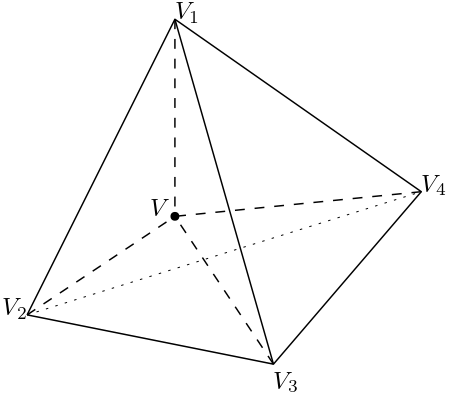
\includegraphics[scale=0.4]{tetraedar2}
  \caption{Točka \textbf{V} definirana z baricentričnimi koordinatami glede na $T$}
  \label{fig:tetraedar2}
\end{figure}
\\V nadaljevanje bomo označevali $\textbf{u} = (u_{1}, u_{2}, u_{3}, u_{4})$. 

\subsection{Domenske točke}
Naj bodo $\textbf{u}$ baricentrične koordinate poljubne točke $(x, y, z)$ glede na izbran tetraeder $T = \langle\textbf{V}_{1}, \textbf{V}_{2}, \textbf{V}_{3}, \textbf{V}_{4}\rangle$. 
Domenske točke Bezierjevega polinoma lahko definiramo kot sledi:
$$
\textbf{X}_{\textbf{i}} = \frac{i}{n}\textbf{V}_{1} + \frac{j}{n}\textbf{V}_{2} + \frac{k}{n}\textbf{V}_{3} + \frac{l}{n}\textbf{V}_{4},
$$
za vsak $\textbf{i} = (i, j, k, l)$ z $|\textbf{i}| = n$.
Baricentrične koordinate domenske točke $\textbf{X}$ 
označimo kot $Bar(\textbf{X}_{\textbf{i}}; T) = \xi^{T}_{\textbf{i}}$.
Za lažjo predstavo si domenske točke oglejmo na sliki \ref{fig:domenske}.

\begin{figure}[h!]
\centering
  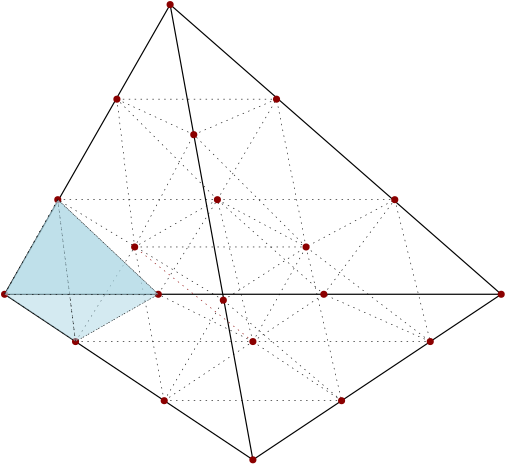
\includegraphics[scale=0.4]{domen}
  \caption{Domenske točke}
  \label{fig:domenske}
\end{figure}

\section{Bernstainovi baznih polinomov treh spremenljivk}
Z notacijo, vpeljano v prejšnjih poglavjih, sedaj definirajmo naslovni 
pojem Bernsteinovih baznih polinomov treh spremenljivk.
\begin{theorem}
  Naj bo $T$ tetraeder in $u_1,u_2,u_3,u_4$
  baricentrične koordinatne funkcije.
  Potem definiramo Bernsteinov bazni polinom treh spremenljivk 
  stopnje $n$ glede na $T$ kot 

  $$
  B_{ijkl}^n := \frac{n!}{i!\text{ }j!\text{ }k!\text{ }l!}u_1^iu_2^ju_3^ku_4^l,\text{    }i+j+k+l=n.
  $$
\end{theorem}

Ob pojavu negativnih indeksov ali indeksov, večjih od $n$, je $B_{ijkl}^n$ enak 0.
Ker so $u_1,u_2,u_3,u_4$ linearni polinomi, sledi,
da je vsak $B_{ijkl}^n$ polinom stopnje $n$. 

\begin{theorem}
  Množica $\mathcal{B}^n := \{B_{ijkl}^n\}_{i+j+k+l=n}$
  Bernsteinovih baznih polinomov predstavlja bazo 
  prostora polinomov treh spremenljivk $\mathbb{P}_n^3$.
  Še več,
  $$
  \sum_{i+j+k+l=n}B^n_{ijkl}(\textbf{u})=1
  \text{ in }
  0\leq B_{ijkl}^n(\textbf{u})\leq 1\text{ }\forall \textbf{u}=\text{Bar}{((x,y,z);T)}, (x,y,z)\in T.$$
\end{theorem}

\begin{proof}
  Da Bernsteinovi bazni polinomi res tvorijo razčlenitev enote, sledi neposredno iz 
  sledečega izračuna:
  $$\sum_{|\textbf{i}|=n}B_{\textbf{i}}^n(\textbf{u})=
  \sum_{|\textbf{i}|=n}\frac{n!}{i!\text{ }j!\text{ }k!\text{ }l!}u_1^iu_2^ju_3^ku_4^l=
  (u_1+u_2+u_3+u_4)^n = 1.
  $$
  Vrednosti $B_{ijkl}^n(\textbf{u})$ se res nahajajo med 0 in 1, 
  saj Bernsteinovi polinomi po definiciji zavzamejo nenegativne vrednosti po eni strani, 
  po drugi pa iz dejstva, da je (kot smo prikazali na začetku tega dokaza) seštevek 
  $B_{ijkl}^n(\textbf{u})$ po vseh $i+j+k+l=n$ enak 1, posamezen Bernsteinov 
  bazni polinom $B_{ijkl}^n(\textbf{u})$ vrednosti 1 gotovo ne bo presegel.

  Dokažimo sedaj, da množica $\mathcal{B}^n$ res predstavlja bazo prostora $\mathbb{P}_n^3$.
  
  Polinomov v množici $\mathcal{B}^n$ je $\binom{n+3}{3}$, kar je enako vrednosti $\dim{\mathbb{P}^3_n}$.
  Preostane nam le še, da z indukcijo pokažemo, 
  da vse monome $\{x^\alpha y^\beta z^\gamma\}_{0\leq \alpha+\beta+\gamma\leq n}$ 
  lahko zapišemo kot linearno kombinacijo Bernstainovih baznih polinomov treh spremenljivk.
  
  Dokazali smo že, da $\sum_{i+j+k+l=n}B^n_{ijkl}(\textbf{u})=1$.
  Če sedaj $x$ najprej razpišemo kot $x=u_1x_1+u_2x_2+u_3x_3+u_4x_4$, nato 
  pa obe strani pomnožimo z
  $1 = \sum_{i+j+k+l=n-1}B_{ijk}^{n-1}$, dobimo:

  $$
  x = \sum_{i+j+k+l=n}\frac{(ix_1+jx_2+kx_3+lx_4)}{n}B_{ijkl}^n(x,y,z).
  $$
  Enak postopek ponovimo še za $y$ in $z$:
  $$
  y = \sum_{i+j+k+l=n}\frac{(iy_1+jy_2+ky_3+ly_4)}{n}B_{ijkl}^n(x,y,z),
  $$
  $$
  z = \sum_{i+j+k+l=n}\frac{(iz_1+jz_2+kz_3+lz_4)}{n}B_{ijkl}^n(x,y,z).
  $$

  Ker je število baznih funkcij v $\mathcal{B}^n$ enako 
  dimenziji $\mathbb{P}_n$, tj. $\binom{n+3}{2}$, sledi, da  
  $\mathcal{B}^n$ predstavlja bazo $\mathbb{P}_n$.
  Sledi 
  $$
  (x,y,z) = 
  \sum_{|\textbf{i}| = n}\bigl(\frac{i}{n}\textbf{V}_1+\frac{j}{n}\textbf{V}_2+\frac{k}{n}\textbf{V}_3+\frac{l}{n}\textbf{V}_4\bigr)B_{\textbf{i}}^n(\textbf{u}),$$
  kjer $\textbf{V}_i = (x_i,y_i,z_i)$.

  Predpostavimo sedaj, da trditev velja vse stopnje, manjše ali enake $n-1$.
  Izberemo monom $x^\alpha y^\beta z^\gamma, \alpha+\beta+\gamma = n$, 
  $c_{\textbf{i}}$ pa predstavlja nek koeficient. Potem:
  \begin{align*}
    &x^\alpha y^\beta z^\gamma = x(x^{\alpha-1} y^\beta z^\gamma) \stackrel{\text{I.P.}}{=} 
    x\sum_{|\textbf{i}|=n}c_{\textbf{i}}B^n_{\textbf{i}}(\textbf{u})\\
    &=(u_1x_1+u_2x_2+u_3x_3+u_4x_4)\sum_{i=0}^{n-1}\Bigl(\sum_{j+k+l=n-1-i}c_{\textbf{i}}\frac{(n-1)!}{i!j!k!l!}u_1^iu_2^ju_3^ku_4^l\Bigr)\\
    &=\dots=\sum_{|\textbf{i}|=n}\bigl(\frac{i}{n}x_1c_{i-1,j,k,l}+x_2c_{i,j,k-1,l}+x_3c_{i,j,k-1,l}+x_4c_{i,j,k,l-1}\bigr)B_{\textbf{i}}^n(\textbf{u})
  \end{align*}
\end{proof}

S tem smo dokazali, da lahko vsak polinom $p\in\mathbb{P}_n^3$ zapišemo kot linearno kombinacijo 
Bernstainovih baznih polinomov treh spremenljivk, torej
$$
p(\textbf{u}) = \sum_{|\textbf{i}|=n}c_{\textbf{i}}B_{\textbf{i}}^n(\textbf{u}).
$$

%\section{Bazna forma (B-forma) polinomov treh spremenljivk}
%Vsak polinom treh spremenljivk se lahko zapiše s pomočjo Bernstainovih baznih polinomov glede na tetraeder $T$. Naj bo $T = \langle\textbf{V}_{1}, \textbf{V}_{2}, \textbf{V}_{3}, \textbf{V}_{4}\rangle$ tetraeder definiran enako kot prej.  
%
%\begin{corollary}
%Vsak polinom $p \in \mathbb{P}^{3}_{n}$ lahko enolično zapišemo v obliki
%\begin{equation} %\label{polinom}
%p(\textbf{u}) = \sum_{i + j + k + l = n}c_{ijkl}B^{n}_{ijkl}(\textbf{u}),
%\end{equation}
%kjer so $\textbf{u} = Bar((x, y, z); T)$, $B^{n}_{ijkl}$ Bernsteinovi baznih polinomov glede na tetraeder $T$ in $c_{ijkl}$ B-koeficienti oz. bazni koeficienti.
%\end{corollary}
%
%Podano imamo kontrolno mrežo, ki je v obliki strukture iz tetraedra. Kontrolne točke označimo z $\textbf{b}_{\textbf{i}} = \textbf{b}_{i,j,k,l}$, $|\textbf{i}| = n$. 
%
%\begin{definicija}
%Bezierov tetraeder stopnje $n$, določen s kontrolnimi točkami $\textbf{b}_{\textbf{i}}$, $|\textbf{i}| = n$ je podan s parametrizacijo
%\begin{equation}
%\textbf{p}(\textbf{u}) = \sum_{|\textbf{i}| = n}\textbf{b}_{\textbf{i}}B_{\textbf{i}}^{n}(\textbf{u}),
%\end{equation}
%kjer je $\textbf{u} = Bar((x, y, z); T)$ in $\textbf{i} = (i, j, k, l)$.
%\end{definicija}

\section{De Casteljaujev algoritam}
Podobno kot pri Bézierjevih krpah lahko točke na Bézierjevih polinomov izračunamo s pomočjo de Casteljaujevega algoritma, ki je posplošitev standardnega de Casteljauovega algoritma za Bézierjeve krivulje. 
Torej lahko izračunamo vrednost Bézierjevega polinoma pri parametar $u$ s ponavljanje linearnih interpolacij. 
Tako kot algoritem za trikotne krpe, imamo tudi tukaj kontrolno mrežo v obliki strukture iz tetraedrov namesto kontrolnega poligona. Kontrolno mrežo določa $\dim\mathbb{P}^{3}_{n} = \binom{n+3}{3} = \frac{(n+3)(n+2)(n+1)}{6}$.

Vhodni podatki algoritma so kontrolnih točk $\textbf{b}_{\textbf{i}}$, $|\textbf{i}| = n$, $i, j, k, l \in \mathbb{N}_{0}$ 
ter točka $(x, y, z)$ z baricentričnimi koordinatam $\textbf{u} = Bar((x,y,z); T)$. 
Izhodni podatek tega algoritma je natančno točka $\textbf{b}_{\textbf{0}}^{n}(\textbf{u}) = \textbf{b}_{0,0,0,0}^{n}$, ki se nahaja na Bezierjevega polinoma. 
Psevdokoda tega algoritma lahko izpišemo kot sledi:

\begin{algorithm}
\caption{de Casteljaujev algoritem}\label{alg:cas}
\begin{algorithmic}
\Require \textbf{$b_{\textbf{i}}$} z $|\textbf{i}| = n$, $\textbf{u} = (u_{1}, u_{2}, u_{3}, u_{4})$
\For{\text{$r = 1, 2, \ldots, n$}}
	\For{$|\textbf{i}| = n-r$}
		\State $\textbf{b}^{r}_{\textbf{i}} = u_{1}\textbf{b}^{r-1}_{i+1,j,k,l} + u_{2}\textbf{b}^{r-1}_{i,j+1,k,l} + u_{3}\textbf{b}^{r-1}_{i,j,k+1,l} + u_{4}\textbf{b}^{r-1}_{i,j,k,l+1}$
	\EndFor
\EndFor
\Ensure $\textbf{b}_{0,0,0,0}^{n}(\textbf{u})$
\end{algorithmic}
\end{algorithm}


\section{Odvodi}

Če imamo podan vektor $\textbf{d} := (d_x,d_y,d_z) \in \mathbb{R}^3$ in točko $\textbf{v} = (x, y, z)$, 
lahko definiramo smerne odvode funkcije treh spremenljivk $f$ v smeri 
vektorja $\textbf{d}$ v točki \textbf{v} kot 
\begin{align*}
  &\left.D_{\textbf{d}}f(x,y,z):=
  \frac{d}{dt}f(\textbf{v}+t\textbf{d})\right|_{t=0}\\
  &=\left.\frac{d}{dt}f(x+td_x,y+td_y,z+td_z)\right|_{t=0}\\
  &=f_x(x,y,z)d_x+f_y(x,y,z)d_y+f_z(x,y,z)d_z.
\end{align*}
Ker pa nas zanimajo odvodi polinomov $p\in\mathbb{P}_n^3$, ki jih izrazimo s pomočjo 
Bernstainovih baznih polinomov, si oglejmo naslednjo lemo.
  \begin{lemma}
        Naj bo $\textbf{d} \in \mathbb{R}^{3}$, 
        Bar(\textbf{d}; T) $= \boldsymbol{\mu} = (\mu_1,\mu_2,\mu_3,\mu_4)$ pa naj predstavljajo 
        njegove baricentrične koordinate. Ker gre za vektor in ne točko, tako velja 
        $\mu_1+\mu_2+\mu_3+\mu_4=0$.
        Potem za poljubne 
        $i+j+k+l=n$ velja:
        \begin{equation*}
          D_{\textbf{d}}B_{ijkl}^n(\textbf{u})
          = n\Bigl(\mu_1B_{i-1,j,k,l}^{n-1}(\textbf{u})+
          \mu_2B_{i,j-1,k,l}^{n-1}(\textbf{u})+
          \mu_3B_{i,j,k-1,l}^{n-1}(\textbf{u})+
          \mu_4B_{i,j,k,l-1}^{n-1}(\textbf{u})
          \Bigr).
        \end{equation*}
    \end{lemma}
    
    \begin{proof}
      Sledimo postopku odvajanja, ki smo ga predstavili na začetku dotičnega poglavja. 
      \begin{align*}
        &D_{\textbf{d}}B_{ijkl}^n(\textbf{u})
        =\left.\frac{d}{dt}B_{\textbf{i}}^n(\textbf{u}+t\boldsymbol{\mu})\right|_{t=0}\\
        &=\left.\frac{d}{dt}\Bigl(\frac{n!}{i!j!k!l!}(u_{1}+t\mu_{1})^{i}(u_{2}+t\mu_{2})^{j}(u_{3}+t\mu_{3})^{k}(u_{4}+t\mu_{4})^{l}\Bigr)\right|_{t=0}\\
        &=\frac{n!}{i!j!k!l!}\Bigl(iu_1^{i-1}u_2^{j}u_3^{k}u_4^{l}\mu_1+ju_1^{i}u_2^{j-1}u_3^{k}u_4^{l}\mu_2+ku_1^{i}u_2^{j}u_3^{k-1}u_4^{l}\mu_3+lu_1^{i}u_2^{j}u_3^{k}u_4^{l-1}\mu_4\Bigr)\\
        &= n\Bigl(\mu_1B_{i-1,j,k,l}^{n-1}(\textbf{u})+
        \mu_2B_{i,j-1,k,l}^{n-1}(\textbf{u})+
        \mu_3B_{i,j,k-1,l}^{n-1}(\textbf{u})+
        \mu_4B_{i,j,k,l-1}^{n-1}(\textbf{u})
        \Bigr).
      \end{align*}
    \end{proof}

    Z uporabo zgornje leme pridemo do naslednjega rezultata:
    $$
    D_{\textbf{d}}p(\textbf{u})= n\sum_{|\textbf{i}|=n-1}\Bigl(\mu_1\textbf{b}_{i+1,j,k,l}+\mu_2\textbf{b}_{i,j+1,k,l}+\mu_3\textbf{b}_{i,j,k+1,l}+\mu_4\textbf{b}_{i,j,k,l+1}\Bigr)B_{\textbf{i}}^{n-1}(\textbf{u})
    $$

    Definirajmo še višje odvode.

    \begin{align*}
      D_{\textbf{d}}^rp(\textbf{u})&=\frac{n!}{(n-r)!}\sum_{|\textbf{i}|=n-r}\textbf{b}_{\textbf{i}}^r(\textbf{u})B_{\textbf{i}}^{n-r}\\
      &=\frac{n!}{(n-r)!}\sum_{|\textbf{i}|=r}\textbf{b}_{\textbf{i}}^{n-r}(\textbf{u})B_{\textbf{i}}^{r}
    \end{align*}

    Za konec omenimo še, da je zaradi neskončne odvedljivosti polinomov 
    v primeru mešanih odvodov (na primer $D_{d_z}D_{d_y}D_{d_x}p(\textbf{u})$) vseeno,
    v kakšnem zaporedju izvajamo posamezne odvode.



% seznam uporabljene literature
\begin{thebibliography}{99}
  \bibitem{1} M. J. Lai, L. Schumaker: Spline functions on triangulations, Cambridge University Press, 2007, str. 434-443.

\end{thebibliography}


\end{document}
